\section{Exact cuts and conditional comparison}\label{sec:discrete}

Throughout this section $x\in[1/\sqrt2,1]$ is fixed. We first work in lattice
units. A finite ambient graph $G=(V,E)$ is a connected induced subgraph of
$\T$ whose bounded faces are elementary triangles and whose union is a
topological disk. We can always take a
large regular hexagon. Holes in a height domain will be represented by fixed
sites in such an ambient graph, rather than by deleting triangles. This
distinction is needed in the wall factorization below.

The cell representation below will provide three conclusions: an exact conditional
factorization across open circuits, order under observations that record a
cell together with all its first-spin sites, and a multiplicative comparison
for separated pin events.  The last comparison remains useful when each pin
event has probability tending to zero.  We first construct the cell law
whose open circuits make all three statements possible.

\subsection{Spins, cells, and exact cuts}

Associate to an integer $H$ the two spins $(B,W)$ given by
\begin{equation}\label{discrete:gray}
\begin{array}{c|cccc}
H\pmod4&0&1&2&3\\ \hline
(B,W)&(+,+)&(+,-)&(-,-)&(-,+).
\end{array}
\end{equation}
Call a spin pair coherent if on each edge at least one of its two spins is
constant. Its free weight on $G$ is
\begin{equation}\label{discrete:pair-weight}
 \prod_{uv\in E}x^{\ind\{(B_u,W_u)\ne(B_v,W_v)\}}\,
 \ind\{(B,W)\text{ is coherent}\}.
\end{equation}
All ambient finite-volume laws in this section use this edge convention.

\begin{lemma}[Integer lift]\label{lem:spin-lift}
Every coherent pair on $G$ has an integer Lipschitz lift, unique up to addition
of a multiple of four once the correspondence \eqref{discrete:gray} is fixed.
For the oriented edge $uv$ its increment is
\begin{equation}\label{discrete:increment}
 H_v-H_u=\frac{W_uB_v-B_uW_v}{2}.
\end{equation}
The free spin law induces the weighted height-increment law with one height
anchored. Fixing a constant pair on a connected skeleton, and fixing the lift
there, induces the usual weighted height Gibbs law in each bounded face of
the skeleton.
\end{lemma}
\begin{proof}
The right side of \eqref{discrete:increment} is $0$, $1$, or $-1$, and has
the required residue in \eqref{discrete:gray}. A triangle cannot have both
spins nonconstant: each nonconstant binary spin changes on two triangle
edges, and these two pairs of edges must intersect. If $B$ is constant on a
triangle, \eqref{discrete:increment} is $-B\,dW/2$ there; if $W$ is constant,
it is $W\,dB/2$. Its circulation therefore vanishes. Every cycle of the
triangulated disk is a sum of its triangle boundaries, so the increments
integrate to $H$. The four choices of the anchor residue give four equally
weighted spin representations of each anchored increment configuration:
cyclic rotation of the states in \eqref{discrete:gray} preserves all
increments and the weight. Finally each disagreeing pair contributes exactly
one factor $x$. Fixing the connected trace fixes the lift on the whole
skeleton, and the remaining edge factors are precisely those of the height
Gibbs specification.
\end{proof}

Let $Y$ be the centers of the upward-pointing elementary triangles, viewed
as one partite class of the dual honeycomb lattice. Each primal edge belongs
to exactly one such triangle. At the ambient boundary a cell can be clipped
to a single edge; cells containing at most one site have no interaction.
For an interacting cell $y$ write $V_y$ for its two or three sites and put
\[
 q_y=\begin{cases}x^2,&|V_y|=3,\\ x,&|V_y|=2.\end{cases}
\]
Introduce an open/closed variable by the following joint weights:
\begin{equation}\label{discrete:cell-table}
\begin{array}{c|c|c}
 \text{status}&\text{allowed spins}&\text{weight}\\ \hline
 \text{open}&B\text{ constant on }V_y,\ W\text{ arbitrary}&q_y\\
 \text{closed}&B,W\text{ both constant on }V_y&1-q_y\\
 \text{closed}&B\text{ nonconstant},\ W\text{ constant on }V_y&q_y.
\end{array}
\end{equation}
An open cell is denoted $+$ or $-$ according to its constant $B$ value,
and a closed cell is denoted $0$; thus $\tau_y\in\{-,0,+\}$.
An interior nonconstant triangle has two changing edges. Summing
\eqref{discrete:cell-table} consequently gives
\eqref{discrete:pair-weight}, including the clipped edge convention.

We permit arbitrary deterministic $B$ pins and deterministic equalities
$W_u=W_v$ on a set $E_0\subset E$. These equalities are not prescribed
component labels. Given $(B,\tau)$, form the graph containing the edges of
all closed cells and all edges of $E_0$, with isolated sites included.
The conditional $W$ law labels its connected components by independent
fair signs. In particular, if $m$ connected subgraphs have already been
required to have constant $W$, the conditional probability that all their
labels are plus lies in $[2^{-m},1]$. This includes singleton subgraphs and
allows several prescribed subgraphs to belong to the same component.

A honeycomb edge is \emph{authorized with sign $s$} if its endpoint in $Y$
has $\tau_y=s$. A good path or circuit of sign $s$ uses authorized edges.
We only use these paths away from clipped ambient cells. The faces adjacent
to a good path have $B=s$ and their connected face chain therefore has a
height trace in one pair of consecutive integers. A nearest-neighbor path
of good $Y$ vertices can be converted into a honeycomb walk by joining
successive vertices through their common honeycomb neighbor. The
displacement is bounded in lattice units. A closed walk with nonzero winding
around a target contains a simple surrounding circuit. All geometric
constructions below have positive clearance, so this conversion preserves
their requirements for sufficiently fine mesh.

\begin{samepage}
\begin{lemma}[Open-cell cut]\label{lem:cell-cut}
Let $\gamma$ be a simple honeycomb circuit strictly inside the ambient graph.
Prescribe $\tau_y=s$ at every $y\in Y\cap\gamma$. Suppose no edge of $E_0$
crosses $\gamma$. Conditional on these prescriptions and any deterministic
constraints on the two respective sides, the two sides are independent
after their prescribed first-spin layers are identified. On the inside,
all cells centered strictly inside retain their original weights; crossing
cells contribute constants and impose no condition on $W$. This inside law
depends only on $\gamma$, $s$, and the constraints inside. Given the complete
height trace of the inside boundary layer, its free sites have the ordinary
weighted height Gibbs law, with any additional inside constraints retained.
\end{lemma}
\end{samepage}
\begin{proof}
Every interacting cell meeting both sides has its honeycomb center on
$\gamma$. Its open prescription fixes every incident first spin to $s$,
and its factor in \eqref{discrete:cell-table} is the constant $q_y$ for
every choice of its second spins. All remaining factors involve sites on
one side only. Equality edges do not cross by assumption. The product
weight and its partition sum thus factor. In particular, complementary
components cannot cross the circuit. After specifying the complete inner
height layer, the spin lift and the edge weights in
Lemma~\ref{lem:spin-lift} give the claimed height specification. No
first-spin agreement event without the open-cell prescriptions has been
used in this factorization.
\end{proof}

\begin{figure}[tbp]
 \centering
 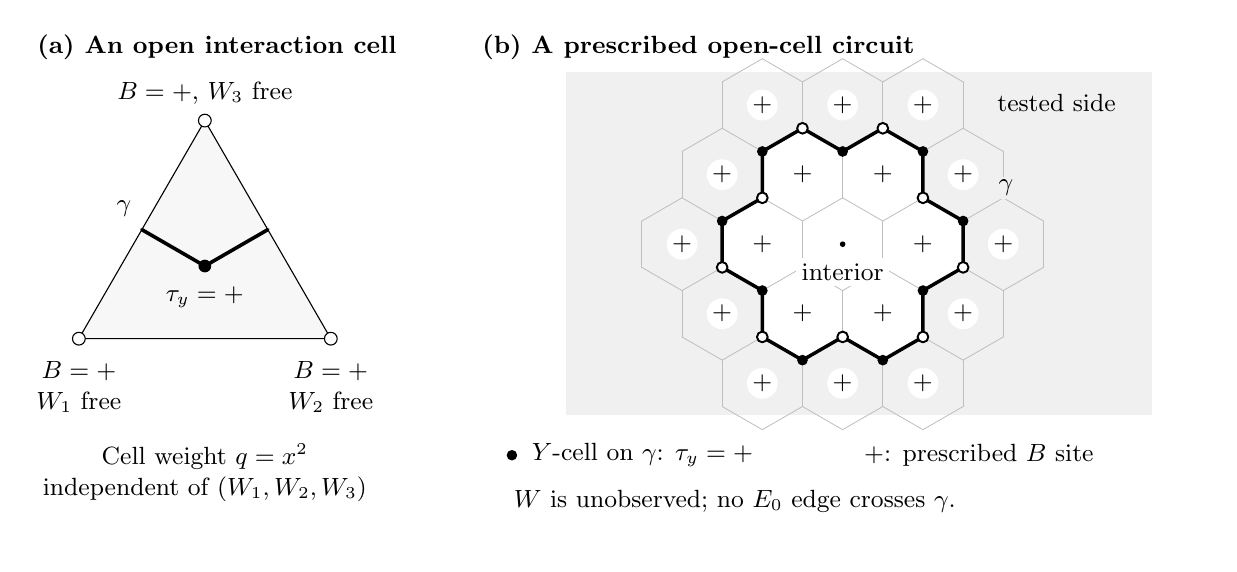
\begin{tikzpicture}[x=1cm,y=1cm,font=\fontsize{9}{11}\selectfont,
  line cap=round,line join=round]
\path[use as bounding box] (0,-1.25) rectangle (15,5.3);
\node[anchor=west,font=\fontsize{9}{11}\selectfont\bfseries] at (0,5.05)
  {(a) An open interaction cell};
\draw[thin,fill=black!3] (0.65,1.35) -- (3.85,1.35) -- (2.25,4.12) -- cycle;
\draw[line width=1.3pt] (1.45,2.735) -- (2.25,2.273) -- (3.05,2.735);
\node[anchor=south east] at (1.44,2.78) {$\gamma$};
\fill (2.25,2.273) circle (2.3pt);
\node[anchor=north] at (2.25,2.13) {$\tau_y=+$};
\foreach \a/\b in {0.65/1.35,3.85/1.35,2.25/4.12}
  \draw[fill=white] (\a,\b) circle (2.3pt);
\node[anchor=south,align=center] at (2.25,4.2) {$B=+$, $W_3$ free};
\node[anchor=north,align=center] at (0.65,1.18) {$B=+$\\$W_1$ free};
\node[anchor=north,align=center] at (3.85,1.18) {$B=+$\\$W_2$ free};
\node[align=center] at (2.25,-0.35)
  {Cell weight $q=x^2$\\independent of $(W_1,W_2,W_3)$};
\node[anchor=west,font=\fontsize{9}{11}\selectfont\bfseries] at (5.65,5.05)
  {(b) A prescribed open-cell circuit};
\begin{scope}[shift={(10.35,2.55)},scale=1.02]
\fill[black!6] (-3.45,-2.13) rectangle (3.85,2.14);
\fill[white] (-1.500000,-0.288675) -- (-1.500000,0.288675) -- (-1.000000,0.577350) -- (-1.000000,1.154701) -- (-0.500000,1.443376) -- (0.000000,1.154701) -- (0.500000,1.443376) -- (1.000000,1.154701) -- (1.000000,0.577350) -- (1.500000,0.288675) -- (1.500000,-0.288675) -- (1.000000,-0.577350) -- (1.000000,-1.154701) -- (0.500000,-1.443376) -- (0.000000,-1.154701) -- (-0.500000,-1.443376) -- (-1.000000,-1.154701) -- (-1.000000,-0.577350) -- cycle;
\draw[black!25,line width=0.3pt] (-2.500000,-0.288675) -- (-2.500000,0.288675);
\draw[black!25,line width=0.3pt] (-2.500000,-0.288675) -- (-2.000000,-0.577350);
\draw[black!25,line width=0.3pt] (-2.500000,0.288675) -- (-2.000000,0.577350);
\draw[black!25,line width=0.3pt] (-2.000000,-1.154701) -- (-2.000000,-0.577350);
\draw[black!25,line width=0.3pt] (-2.000000,-1.154701) -- (-1.500000,-1.443376);
\draw[black!25,line width=0.3pt] (-2.000000,-0.577350) -- (-1.500000,-0.288675);
\draw[black!25,line width=0.3pt] (-2.000000,0.577350) -- (-2.000000,1.154701);
\draw[black!25,line width=0.3pt] (-2.000000,0.577350) -- (-1.500000,0.288675);
\draw[black!25,line width=0.3pt] (-2.000000,1.154701) -- (-1.500000,1.443376);
\draw[black!25,line width=0.3pt] (-1.500000,-2.020726) -- (-1.500000,-1.443376);
\draw[black!25,line width=0.3pt] (-1.500000,-2.020726) -- (-1.000000,-2.309401);
\draw[black!25,line width=0.3pt] (-1.500000,-1.443376) -- (-1.000000,-1.154701);
\draw[black!25,line width=0.3pt] (-1.500000,-0.288675) -- (-1.500000,0.288675);
\draw[black!25,line width=0.3pt] (-1.500000,-0.288675) -- (-1.000000,-0.577350);
\draw[black!25,line width=0.3pt] (-1.500000,0.288675) -- (-1.000000,0.577350);
\draw[black!25,line width=0.3pt] (-1.500000,1.443376) -- (-1.500000,2.020726);
\draw[black!25,line width=0.3pt] (-1.500000,1.443376) -- (-1.000000,1.154701);
\draw[black!25,line width=0.3pt] (-1.500000,2.020726) -- (-1.000000,2.309401);
\draw[black!25,line width=0.3pt] (-1.000000,-2.309401) -- (-0.500000,-2.020726);
\draw[black!25,line width=0.3pt] (-1.000000,-1.154701) -- (-1.000000,-0.577350);
\draw[black!25,line width=0.3pt] (-1.000000,-1.154701) -- (-0.500000,-1.443376);
\draw[black!25,line width=0.3pt] (-1.000000,-0.577350) -- (-0.500000,-0.288675);
\draw[black!25,line width=0.3pt] (-1.000000,0.577350) -- (-1.000000,1.154701);
\draw[black!25,line width=0.3pt] (-1.000000,0.577350) -- (-0.500000,0.288675);
\draw[black!25,line width=0.3pt] (-1.000000,1.154701) -- (-0.500000,1.443376);
\draw[black!25,line width=0.3pt] (-1.000000,2.309401) -- (-0.500000,2.020726);
\draw[black!25,line width=0.3pt] (-0.500000,-2.020726) -- (-0.500000,-1.443376);
\draw[black!25,line width=0.3pt] (-0.500000,-2.020726) -- (0.000000,-2.309401);
\draw[black!25,line width=0.3pt] (-0.500000,-1.443376) -- (0.000000,-1.154701);
\draw[black!25,line width=0.3pt] (-0.500000,-0.288675) -- (-0.500000,0.288675);
\draw[black!25,line width=0.3pt] (-0.500000,-0.288675) -- (0.000000,-0.577350);
\draw[black!25,line width=0.3pt] (-0.500000,0.288675) -- (0.000000,0.577350);
\draw[black!25,line width=0.3pt] (-0.500000,1.443376) -- (-0.500000,2.020726);
\draw[black!25,line width=0.3pt] (-0.500000,1.443376) -- (0.000000,1.154701);
\draw[black!25,line width=0.3pt] (-0.500000,2.020726) -- (0.000000,2.309401);
\draw[black!25,line width=0.3pt] (0.000000,-2.309401) -- (0.500000,-2.020726);
\draw[black!25,line width=0.3pt] (0.000000,-1.154701) -- (0.000000,-0.577350);
\draw[black!25,line width=0.3pt] (0.000000,-1.154701) -- (0.500000,-1.443376);
\draw[black!25,line width=0.3pt] (0.000000,-0.577350) -- (0.500000,-0.288675);
\draw[black!25,line width=0.3pt] (0.000000,0.577350) -- (0.000000,1.154701);
\draw[black!25,line width=0.3pt] (0.000000,0.577350) -- (0.500000,0.288675);
\draw[black!25,line width=0.3pt] (0.000000,1.154701) -- (0.500000,1.443376);
\draw[black!25,line width=0.3pt] (0.000000,2.309401) -- (0.500000,2.020726);
\draw[black!25,line width=0.3pt] (0.500000,-2.020726) -- (0.500000,-1.443376);
\draw[black!25,line width=0.3pt] (0.500000,-2.020726) -- (1.000000,-2.309401);
\draw[black!25,line width=0.3pt] (0.500000,-1.443376) -- (1.000000,-1.154701);
\draw[black!25,line width=0.3pt] (0.500000,-0.288675) -- (0.500000,0.288675);
\draw[black!25,line width=0.3pt] (0.500000,-0.288675) -- (1.000000,-0.577350);
\draw[black!25,line width=0.3pt] (0.500000,0.288675) -- (1.000000,0.577350);
\draw[black!25,line width=0.3pt] (0.500000,1.443376) -- (0.500000,2.020726);
\draw[black!25,line width=0.3pt] (0.500000,1.443376) -- (1.000000,1.154701);
\draw[black!25,line width=0.3pt] (0.500000,2.020726) -- (1.000000,2.309401);
\draw[black!25,line width=0.3pt] (1.000000,-2.309401) -- (1.500000,-2.020726);
\draw[black!25,line width=0.3pt] (1.000000,-1.154701) -- (1.000000,-0.577350);
\draw[black!25,line width=0.3pt] (1.000000,-1.154701) -- (1.500000,-1.443376);
\draw[black!25,line width=0.3pt] (1.000000,-0.577350) -- (1.500000,-0.288675);
\draw[black!25,line width=0.3pt] (1.000000,0.577350) -- (1.000000,1.154701);
\draw[black!25,line width=0.3pt] (1.000000,0.577350) -- (1.500000,0.288675);
\draw[black!25,line width=0.3pt] (1.000000,1.154701) -- (1.500000,1.443376);
\draw[black!25,line width=0.3pt] (1.000000,2.309401) -- (1.500000,2.020726);
\draw[black!25,line width=0.3pt] (1.500000,-2.020726) -- (1.500000,-1.443376);
\draw[black!25,line width=0.3pt] (1.500000,-1.443376) -- (2.000000,-1.154701);
\draw[black!25,line width=0.3pt] (1.500000,-0.288675) -- (1.500000,0.288675);
\draw[black!25,line width=0.3pt] (1.500000,-0.288675) -- (2.000000,-0.577350);
\draw[black!25,line width=0.3pt] (1.500000,0.288675) -- (2.000000,0.577350);
\draw[black!25,line width=0.3pt] (1.500000,1.443376) -- (1.500000,2.020726);
\draw[black!25,line width=0.3pt] (1.500000,1.443376) -- (2.000000,1.154701);
\draw[black!25,line width=0.3pt] (2.000000,-1.154701) -- (2.000000,-0.577350);
\draw[black!25,line width=0.3pt] (2.000000,-0.577350) -- (2.500000,-0.288675);
\draw[black!25,line width=0.3pt] (2.000000,0.577350) -- (2.000000,1.154701);
\draw[black!25,line width=0.3pt] (2.000000,0.577350) -- (2.500000,0.288675);
\draw[black!25,line width=0.3pt] (2.500000,-0.288675) -- (2.500000,0.288675);
\draw[line width=1.25pt] (-1.500000,-0.288675) -- (-1.500000,0.288675) -- (-1.000000,0.577350) -- (-1.000000,1.154701) -- (-0.500000,1.443376) -- (0.000000,1.154701) -- (0.500000,1.443376) -- (1.000000,1.154701) -- (1.000000,0.577350) -- (1.500000,0.288675) -- (1.500000,-0.288675) -- (1.000000,-0.577350) -- (1.000000,-1.154701) -- (0.500000,-1.443376) -- (0.000000,-1.154701) -- (-0.500000,-1.443376) -- (-1.000000,-1.154701) -- (-1.000000,-0.577350) -- cycle;
\draw[fill=white,line width=0.7pt] (-1.500000,-0.288675) circle (1.9pt);
\fill (-1.500000,0.288675) circle (1.9pt);
\draw[fill=white,line width=0.7pt] (-1.000000,0.577350) circle (1.9pt);
\fill (-1.000000,1.154701) circle (1.9pt);
\draw[fill=white,line width=0.7pt] (-0.500000,1.443376) circle (1.9pt);
\fill (0.000000,1.154701) circle (1.9pt);
\draw[fill=white,line width=0.7pt] (0.500000,1.443376) circle (1.9pt);
\fill (1.000000,1.154701) circle (1.9pt);
\draw[fill=white,line width=0.7pt] (1.000000,0.577350) circle (1.9pt);
\fill (1.500000,0.288675) circle (1.9pt);
\draw[fill=white,line width=0.7pt] (1.500000,-0.288675) circle (1.9pt);
\fill (1.000000,-0.577350) circle (1.9pt);
\draw[fill=white,line width=0.7pt] (1.000000,-1.154701) circle (1.9pt);
\fill (0.500000,-1.443376) circle (1.9pt);
\draw[fill=white,line width=0.7pt] (0.000000,-1.154701) circle (1.9pt);
\fill (-0.500000,-1.443376) circle (1.9pt);
\draw[fill=white,line width=0.7pt] (-1.000000,-1.154701) circle (1.9pt);
\fill (-1.000000,-0.577350) circle (1.9pt);
\node[font=\fontsize{9}{11}\selectfont,inner sep=0.6pt,circle,fill=white] at (-2.000000,0.000000) {$+$};
\node[font=\fontsize{9}{11}\selectfont,inner sep=0.6pt,circle,fill=white] at (-1.500000,0.866025) {$+$};
\node[font=\fontsize{9}{11}\selectfont,inner sep=0.6pt,circle,fill=white] at (-1.000000,1.732051) {$+$};
\node[font=\fontsize{9}{11}\selectfont,inner sep=0.6pt,circle,fill=white] at (-1.500000,-0.866025) {$+$};
\node[font=\fontsize{9}{11}\selectfont,inner sep=0.6pt,circle,fill=white] at (-1.000000,0.000000) {$+$};
\node[font=\fontsize{9}{11}\selectfont,inner sep=0.6pt,circle,fill=white] at (-0.500000,0.866025) {$+$};
\node[font=\fontsize{9}{11}\selectfont,inner sep=0.6pt,circle,fill=white] at (0.000000,1.732051) {$+$};
\node[font=\fontsize{9}{11}\selectfont,inner sep=0.6pt,circle,fill=white] at (-1.000000,-1.732051) {$+$};
\node[font=\fontsize{9}{11}\selectfont,inner sep=0.6pt,circle,fill=white] at (-0.500000,-0.866025) {$+$};
\fill (0.000000,0.000000) circle (1pt);
\node[font=\fontsize{9}{11}\selectfont,inner sep=0.6pt,circle,fill=white] at (0.500000,0.866025) {$+$};
\node[font=\fontsize{9}{11}\selectfont,inner sep=0.6pt,circle,fill=white] at (1.000000,1.732051) {$+$};
\node[font=\fontsize{9}{11}\selectfont,inner sep=0.6pt,circle,fill=white] at (0.000000,-1.732051) {$+$};
\node[font=\fontsize{9}{11}\selectfont,inner sep=0.6pt,circle,fill=white] at (0.500000,-0.866025) {$+$};
\node[font=\fontsize{9}{11}\selectfont,inner sep=0.6pt,circle,fill=white] at (1.000000,0.000000) {$+$};
\node[font=\fontsize{9}{11}\selectfont,inner sep=0.6pt,circle,fill=white] at (1.500000,0.866025) {$+$};
\node[font=\fontsize{9}{11}\selectfont,inner sep=0.6pt,circle,fill=white] at (1.000000,-1.732051) {$+$};
\node[font=\fontsize{9}{11}\selectfont,inner sep=0.6pt,circle,fill=white] at (1.500000,-0.866025) {$+$};
\node[font=\fontsize{9}{11}\selectfont,inner sep=0.6pt,circle,fill=white] at (2.000000,0.000000) {$+$};
\node[fill=white,inner sep=2pt] at (0,-0.35) {interior};
\node[anchor=west,fill=black!6,inner sep=2pt] at (1.85,1.76) {tested side};
\node[anchor=west,fill=black!6,inner sep=1pt] at (1.9,0.7) {$\gamma$};
\end{scope}
\fill (6.15,-0.13) circle (1.9pt);
\node[anchor=west] at (6.28,-0.13) {$Y$-cell on $\gamma$: $\tau_y=+$};
\node[anchor=west] at (10.5,-0.13) {$+$: prescribed $B$ site};
\node[anchor=west] at (6.05,-0.72)
  {$W$ is unobserved; no $E_0$ edge crosses $\gamma$.};
\end{tikzpicture}

 \caption{An exact open-cell cut. In (a), prescribing $B=+$ and
 $\tau_y=+$ gives the constant cell weight $q=x^2$ for every second-spin
 assignment. In (b), filled circuit vertices are open-plus $Y$ cells;
 plus signs mark their prescribed first-spin sites. The tested exterior
 is shaded. No equality edge crosses $\gamma$, and the unobserved second
 spins have no component joining its two sides. Strictly interior cells
 retain their original interactions.}
 \label{discrete:fig-cut}
\end{figure}

\begin{samepage}
Here is the only crossing estimate imported into the discrete argument.
The boundary convention in its statement is part of the theorem.

\begin{theorem}[Glazman--Lammers circuit input]\label{thm:circuit-input}
For $r\ge0$, let $\Lambda_r$ be the ball of radius $r$ in the triangular
graph metric, with its bounding honeycomb contour; thus
$\Lambda_r=\Lambda_{\lfloor r\rfloor}$. For $a>1$ and an integer
$n\in\N$, consider on
$\Lambda_{an}$ the cell spin law whose
interior cells have weight $(x^2)^{\ind\{B\text{ or }W\text{ nonconstant}\}}$
and whose boundary $Y$ cells are excluded. Fix $B=-$ on the boundary face
layer and leave $W$ free. There is $c=c(x,a)>0$ such
that, for $n\ge 3/(a-1)$, the probability of an occupied open-plus cell
circuit surrounding $\Lambda_n$ and contained in $\Lambda_{an}$ is at
least $c$. The same statement holds with the signs or the two spin colors
interchanged.
\end{theorem}
\end{samepage}

This is equation (55) in Appendix A of the third arXiv version of
\cite{GL2025}, with Definitions 3.2 and 3.5. Its augmentation includes a
cell whenever $W$ is nonconstant, excludes it whenever $B$ is nonconstant,
and otherwise includes it with probability $x^2$. It is therefore exactly
\eqref{discrete:cell-table}. The source uses
$Y(\Omega)=(Y\cap V(\Omega))\setminus V(\partial\Omega)$; simply pinning
$B=-$ in our edge-weight law would still charge certain boundary $W$
changes. Lemma~\ref{lem:cell-cut} instead identifies the source law with
the law inside a prescribed regular open-minus circuit: the excluded
boundary factors become constants. This is also the conditional law
described by Lemma 3.8 of \cite{GL2025}. We use the theorem only through
this exact identification, with fixed slack for lattice rounding. In
particular its validity includes $x=1/\sqrt2$.

\subsection{Restricted histories and the two-law inequality}

A \emph{history} fixes some first-spin sites and some cell statuses, with
the rule that it fixes \emph{all} first-spin sites of every observed cell.
The equality set $E_0$ remains deterministic. No second-spin component
labels are part of a history. Order first spins by $-<+$ and statuses by
$-<0<+$. Ordered histories have the same observation sets and ordered
values. They may also have additional deterministic plus $B$ pins only in
the upper law, or additional deterministic minus $B$ pins only in the
lower law, compatible with the common pins.

\begin{proposition}[Association and conditional order]\label{prop:history-order}
For every feasible history, the unobserved $(B,\tau)$ variables are
positively associated. Two laws with ordered histories and common $E_0$
are stochastically ordered, including the unequal extreme pins just
described. Extra prescribed open-plus cells only in the upper law, or
open-minus cells only in the lower law, can be incorporated by observing
those cells and all their first-spin sites also in the other law. These
claims hold for clipped cells and at $x=1$.
\end{proposition}

We first prove two finite-weight inequalities used in the proof of this
proposition, then apply them to the cell law.

We use the finite association inequality of Fortuin--Kasteleyn--Ginibre
\cite{FKG1971}, including weights that vanish.  Its precise form follows
from the rounded-midpoint inequality stated and tensorized in
Theorem~\ref{thm:midpoint}: for nonnegative finitely supported arrays,
the premise
$f(b)g(c)\le u(\lfloor(b+c)/2\rfloor)v(\lceil(b+c)/2\rceil)$
implies $(\sum f)(\sum g)\le(\sum u)(\sum v)$.
Indeed, on a Boolean cube the rounded
midpoints of $b,c$ are their coordinatewise minimum $b\wedge c$ and
maximum $b\vee c$.  If a nonnegative weight $w$ satisfies
$w(b)w(c)\le w(b\wedge c)w(b\vee c)$ and $F,G$ are nonnegative
increasing functions, then
\[
 w(b)F(b)w(c)G(c)
 \le w(b\wedge c)w(b\vee c)F(b\vee c)G(b\vee c).
\]
Apply the midpoint inequality to $wF,wG,w,wFG$, extended by zero
outside the cube.  Its conclusion is
$(\sum wF)(\sum wG)\le(\sum w)(\sum wFG)$, which is association
after normalization.  Encode an element of a finite chain by a prefix
of ones followed by zeros.  The encoded product of chains is closed
under minimum and maximum, so extension by zero proves the same result
there.  Adding constants to bounded increasing functions covers signed
functions.  This deduction explains every finite association use below;
the midpoint tensorization itself uses no association statement.

The wall decomposition below expresses the first-spin weight using two
partition sums for the complementary spin.  We record the two properties
of those sums needed to compare first-spin configurations.

\begin{lemma}[The complementary-spin partition sum]
\label{discrete:ising-partition}
For $a\in[0,1]^E$ define
\begin{equation}\label{discrete:ising-Z}
 Z(a)=\sum_{\sigma\in\{-,+\}^{V}}
             \prod_{e=uv\in E}a_e^{\ind\{\sigma_u\ne\sigma_v\}},
 \qquad 0^0=1.
\end{equation}
Then $Z$ is increasing in every coordinate and is log-supermodular:
\begin{equation}\label{discrete:Z-lattice}
 Z(a\wedge b)Z(a\vee b)\ge Z(a)Z(b).
\end{equation}
\end{lemma}
\begin{proof}
Monotonicity follows term by term.  For positive coordinates the second assertion follows by differentiating in $\log a_e$.
For distinct edges $e=uv$ and $f=st$,
\[
 \frac{\partial^2\log Z}{\partial\log a_e\,\partial\log a_f}
 =\Cov(\ind\{\sigma_u\ne\sigma_v\},
              \ind\{\sigma_s\ne\sigma_t\})
 =\tfrac14\Cov(\sigma_u\sigma_v,\sigma_s\sigma_t)\ge0.
\]
The last inequality is a special case of the second Griffiths inequality
\cite{GKS1968}; we recall its random-cluster proof \cite[p.~102]{FKG1971}. Put
$J_e=-\frac12\log a_e\ge0$ and $p_e=1-e^{-2J_e}=1-a_e$. Expanding
\[
 e^{J_e\sigma_u\sigma_v}
 =e^{J_e}\bigl((1-p_e)+p_e\ind\{\sigma_u=\sigma_v\}\bigr)
\]
over edges gives a joint spin--bond law whose bond marginal on
$\omega\subset E$ has weight
\[
 2^{k(\omega)}\prod_{e\in\omega}p_e
                    \prod_{e\notin\omega}(1-p_e),
\]
where $k(\omega)$ counts all connected components, including isolated
vertices. This weight satisfies the lattice condition. Indeed, if
$\mathcal C(A)$ is the binary cycle space of the edge set $A$, then
$\mathcal C(A)\cap\mathcal C(B)=\mathcal C(A\cap B)$ and
$\mathcal C(A)+\mathcal C(B)\subset\mathcal C(A\cup B)$.
Taking dimensions and using
$k(A)=|V|-|A|+\dim\mathcal C(A)$ proves supermodularity of $k$;
the remaining edge factors are modular. The FKG theorem
\cite{FKG1971} therefore associates increasing bond events.
Conditional on $\omega$, the spins are independent fair signs on its
components. Consequently
$\E(\sigma_u\sigma_v)=\Prob(u\leftrightarrow v)$, while the
conditional expectation of $\sigma_u\sigma_v\sigma_s\sigma_t$ is
one precisely when each component contains an even number of the four
listed vertices, counted with multiplicity, and is zero otherwise. In
particular
\[
 \E(\sigma_u\sigma_v\sigma_s\sigma_t)
 \ge\Prob(u\leftrightarrow v,\ s\leftrightarrow t)
 \ge\Prob(u\leftrightarrow v)\Prob(s\leftrightarrow t).
\]
This proves the required covariance inequality, also when the edges share
vertices. The cases $p_e\in\{0,1\}$ follow by continuity. Integrating
the nonnegative mixed derivatives over coordinate rectangles gives
\eqref{discrete:Z-lattice}; continuity of the polynomial $Z$ includes its
zero-coordinate cases.

\end{proof}


\begin{proof}[Proof of Proposition~\ref{prop:history-order}]
We first sum the second spins by splitting their walls according to the
first-spin sign.  Lemma~\ref{discrete:ising-partition} will give the
two-law inequality for this marginal.  We then restore the statuses.

Fix a first-spin configuration $b$. A binary edge set is a second-spin
wall precisely when it has even intersection with every triangle boundary.
Indeed this condition makes its mod-two integral independent of the path
from a fixed anchor, since triangle boundaries generate the cycle space.
There are exactly two spin labelings for each such wall. Every allowed wall
edge has homogeneous $b$ endpoints. Split these edges according to their
common sign. A homogeneous triangle has only one sign class. A mixed
triangle has just one homogeneous edge, which its even rule forces to be
absent. Thus none of the triangle equations couples the two sign classes.
Each sign restriction of an allowed wall is itself a wall, and arbitrary
walls supported in the two allowed sign sets can be combined. This proves
factorization without an additional global compatibility condition.

For an unobserved cell let
$r_y(b)=1$ if $b$ is homogeneous there and $r_y(b)=q_y$ otherwise.
Define $a_h^+(b)$ as follows: it equals $x$ on edges of unobserved
homogeneous-plus cells, equals $1$ on observed open-plus cells, and is zero
on all other edges. Set it to zero also on $E_0$. Define $a_h^-(b)$ with
minus in place of plus. Summing the unobserved statuses and then the second
spins gives the first-spin weight
\begin{equation}\label{discrete:wall-factor}
 w_h(b)=\frac{c_h}{2}\,
   \prod_{y\text{ unobserved}}r_y(b)\,
   Z(a_h^+(b))Z(a_h^-(b))\,
   \ind\{b\text{ satisfies its fixed sites}\}.
\end{equation}
Here $c_h>0$ is the product of the observed-cell factors; these are
constants because their first spins are fixed. The factor $1/2$ is exact:
each $Z$ counts two global signs whereas the actual second-spin sum counts
only two, not four. In particular $E_0$ deletes wall coordinates and does
not impose a relation between the two global signs. Formula
\eqref{discrete:wall-factor} would in general fail on a graph with a hole
if the missing cycle constraints were omitted, explaining our ambient
triangulation convention.

Let $h_-\le h_+$ be ordered histories. For any $b$ in the lower support and
$c$ in the upper support, $b\wedge c$ belongs to the lower support and
$b\vee c$ to the upper support, also when pins occur in just one law.
On an unobserved cell, homogeneous-plus eligibility at the meet is the
intersection of the input eligibilities; at the join it contains their
union. Therefore, coordinatewise,
\begin{align*}
 a_{h_-}^+(b\wedge c)&\ge a_{h_-}^+(b)\wedge a_{h_+}^+(c),&
 a_{h_+}^+(b\vee c)&\ge a_{h_-}^+(b)\vee a_{h_+}^+(c),\\
 a_{h_-}^-(b\wedge c)&\ge a_{h_-}^-(b)\vee a_{h_+}^-(c),&
 a_{h_+}^-(b\vee c)&\ge a_{h_-}^-(b)\wedge a_{h_+}^-(c).
\end{align*}
On observed cells the plus vectors are already ordered and the minus
vectors reverse-ordered; hence the same inequalities hold there. Deleting
the common coordinates $E_0$ preserves all four inequalities.
Furthermore
\[
 r_y(b\wedge c)r_y(b\vee c)\ge r_y(b)r_y(c).
\]
To check this last assertion, comparable restrictions are unchanged by
sorting. For incomparable restrictions both inputs are mixed, whereas
each output has weight at least $q_y$. A homogeneous input is extremal
and cannot be lost. Applying monotonicity and
\eqref{discrete:Z-lattice} to each sign in
\eqref{discrete:wall-factor} now proves
\begin{equation}\label{discrete:two-law}
 w_{h_-}(b\wedge c)w_{h_+}(b\vee c)
       \ge w_{h_-}(b)w_{h_+}(c).
\end{equation}
Observed-cell constants cancel. This also proves the lattice condition
within either first-spin law.

For clarity, zero weights and unequal supports cause no invocation of an
unstated strictly positive version of Holley's criterion
\cite{Holley1974}. Extend the weights by zero to the whole first-spin cube
and put $\widetilde w(b,0)=w_{h_-}(b)$,
$\widetilde w(b,1)=w_{h_+}(b)$. The two within-layer inequalities and
\eqref{discrete:two-law} say that $\widetilde w$ satisfies the lattice
condition on the cube times $\{0,1\}$. The nonnegative-weight FKG theorem
\cite{FKG1971} applies. For increasing $f$, its positive covariance with
the last coordinate says exactly
$\E_{h_-}f(B)\le\E_{h_+}f(B)$. The same theorem gives association of
each first-spin law. This proves the needed extension to sorted supports.

It remains to restore statuses. Given $b$, each unobserved homogeneous
cell is eligible to open with its sign; mixed cells are necessarily closed.
Let $S_+$ and $S_-$ be the two open subsets of eligible cells. Wall
factorization now gives independent weights for these subsets. Apart from
constants their respective weights are
\begin{equation}\label{discrete:subset-weight}
 \prod_{y\in S_s}q_y
 \prod_{y\in I_s\setminus S_s}(1-q_y)\,
 Z\bigl(\ind\{e\text{ lies in an open cell of sign }s\}
                    \ind\{e\notin E_0\}\bigr),
\end{equation}
where $I_s$ is the eligible set and observed open cells of sign $s$ are
included as fixed allowed cells in the last factor. Different cells have
disjoint edge sets. The Bernoulli factor is modular; the $Z$ factor is
log-supermodular in the cell set by \eqref{discrete:Z-lattice}. Thus each
subset law is associated. The same two-law calculation shows stochastic
increase under enlarging $I_s$ or the fixed allowed cells: on a common
subset cube the sorted allowed-edge sets contain the coordinatewise
intersection and union, and the Bernoulli factors cancel. Ineligible cells
are held closed. The preceding nonnegative-weight argument again handles
these deterministic restrictions.

Increasing $b$ enlarges plus eligibility and shrinks minus eligibility.
Hence $S_+$ increases and $S_-$ decreases in inclusion order, exactly the
status order $-<0<+$. Association of the minus block is also association
in reverse inclusion order, since the covariance of decreasing functions
equals that of their negatives. The two blocks are independent. If $F,G$
are increasing functions of $(B,\tau)$, conditional association gives
$\E(FG\mid B)\ge\E(F\mid B)\E(G\mid B)$; the two conditional
expectations are increasing in $B$. Association of $B$ completes the
joint association claim. An ordered coupling of the first spins followed
by ordered conditional status kernels gives the two-law assertion.

If $q_y=1$, a homogeneous unobserved cell is open deterministically, and
an observed homogeneous closed cell is infeasible. All displayed
inequalities remain valid on feasible supports, either directly or by
continuity as $q_y\uparrow1$; no division by $1-q_y$ is used. Finally an
extra open-plus cell in the upper law has the maximum possible status and
first-spin values. Querying that same block in the lower law always gives
ordered values and retains its correct distribution. This is observation
in the other law, not imposition of the upper event on it. The open-minus
case is symmetric.
\end{proof}

\begin{remark}\label{discrete:not-raw-FKG}
Proposition~\ref{prop:history-order} asserts association of the joint law,
not the lattice condition for its unsummed density. Nor does it allow
observation of a closed status without its first spins. For example, on a
single triangle conditioned only to be closed, the first-spin weight is
$1-q$ on the two homogeneous configurations and $q$ on the six mixed
ones. Its pair covariance is $(1-2q)/(1+2q)<0$ when $q>1/2$.
\end{remark}

\subsection{Online exploration and buffered circuits}

We next specify the probabilistic meaning of coupled exploration. This
will matter again when the remaining interior is compared with a plane
sample independent of exterior observables.

\begin{lemma}[Conditional kernels at a joint record]\label{discrete:online}
Consider two finite-volume laws ordered as in
Proposition~\ref{prop:history-order}. There is an online exploration
coupling with the following invariant: conditional on every full joint
query record, the eventual completion in either coordinate has that
coordinate's original Gibbs conditional law given its own observed values
and deterministic constraints. The next cell, together with all its first
spins, may be chosen as any deterministic function of the joint record.
If the retained conditional problems become identical, their completions
can be sampled identically.
\end{lemma}
\begin{proof}
At a joint record $R$ let $\mu_i^R$ be the two specified own-history
conditional laws. Select a common query block $Q=Q(R)$ and couple its
marginals by an ordered kernel $\kappa_R$, available from
Proposition~\ref{prop:history-order}. For each possible pair of answers
$(a_1,a_2)$ recursively complete with the respective conditional laws
$\mu_i^R(\cdot\mid Q=a_i)$. This is a finite recursion: every nonterminal
query adds a new cell or site. At a terminal node with the same remaining
specification, use one draw from that common law. At any other terminal
node use any coupling of its two remaining laws.

Backward induction proves the marginal invariant. For a completed
observable $f$ in coordinate $1$, the expectation from the node $R$ is
\[
 \sum_{a_1,a_2}\kappa_R(a_1,a_2)
       \mu_1^R(f\mid Q=a_1)
 =\sum_{a_1}\mu_1^R(Q=a_1)\mu_1^R(f\mid Q=a_1)
 =\mu_1^R(f).
\]
The second coordinate is identical. Applying the same induction starting
at any reached node gives the assertion conditional on the whole joint
record, not merely on an individual history. Independent randomness used
to select a query can be put in the record and conditioned on first.
No conditioning of a previously sampled full-field coupling is involved.
\end{proof}

The following geometric exploration implements the lemma. In a prescribed
annular search area authorize the honeycomb edges incident to favorable
open $Y$ cells; edges outside the area may be declared unavailable. Start
from the exterior face set for an inward search, or from a connected inner
face layer for an outward search. Invade across unauthorized honeycomb
edges, querying the responsible cell and its full first-spin block in both
laws when needed. On reaching a prescribed authorized circuit with
clearance the invasion cannot cross it. The boundary of the invaded union
of honeycomb faces consists of authorized contours. Select the component
separating the start from the protected target, deleting inessential
excursions to obtain a simple circuit. In an inward search this is the
boundary around the component containing the connected target; in an
outward search it is the outer boundary of the invaded set.

There is no hidden revelation on the retained side. A queried cell touches
the invaded face set. A honeycomb vertex strictly on one side of an edge
contour touches only faces on that side. A queried cell meeting both sides
therefore lies on the contour and is favorable open, so its retained
first-spin sites have the prescribed contour sign. If a queried cell is
not favorable, invasion crosses all its incident unauthorized edges; it
cannot leave an unprescribed first-spin neighbor behind that cell. Thus
the only retained sites queried are prescribed cut-layer first spins.
Second-spin labels remain unqueried. In the absence of crossing $E_0$
edges, Lemma~\ref{lem:cell-cut} identifies the stopped retained law.
Together with Lemma~\ref{discrete:online}, this proves the exact stopped-cut
and common-sampling assertions for either direction of exploration.

\begin{lemma}[Buffered circuits and paths]\label{lem:buffer-circuits}
Fix a finite collection of annuli and tubes in a bounded planar region,
each with a positive-width buffer and with prescribed geometric clearance.
At mesh $\delta$, suppose the buffers contain no equality edge $E_0$ and
no first-spin pin adverse to a requested sign. Then each request for good
circuits, or connected good paths formed from a finite annular chain, has
probability bounded below by a positive constant independent of $\delta$
for all sufficiently small $\delta$. The bound is uniform over feasible
histories supported away from the buffers and over lattice translations
preserving the clearances. Requests with the same sign may be combined by
association; requests of different signs in disjoint buffers may be made
successively. In an annular stack of fixed-ratio, separated slots between
lattice scales $r$ and $L$, the probability of finding no requested good
circuit is at most
\begin{equation}\label{discrete:stack}
 C(r/L)^\alpha,
\end{equation}
for constants $C,\alpha>0$.

Moreover, conditioning a free ambient law on any deterministic collection
of open-plus cells and their first-spin values increases every increasing
event in $(B,\tau)$. This applies to a favorable path event in the ambient
plane even when its path leaves the interior of a prescribed good contour.
\end{lemma}
\begin{proof}
The primitive comparison takes place in a small \emph{filled} regular
disk whose entire larger comparison cut and interior fit inside the
buffer. In that disk consider a smaller regular annulus. Delete
favorable pins in the filled disk, which
can only decrease the probability of the favorable increasing event.
Prescribing the outer cut open with the adverse sign decreases it again
by Proposition~\ref{prop:history-order}. There are no other constraints
inside this small outer cut. Lemma~\ref{lem:cell-cut} and
Theorem~\ref{thm:circuit-input} give a positive lower bound in the
resulting deterministic regular problem. The same comparison applies
after any allowed outside history. For a minus request reverse all first
spins and the status order.

For gluing, use regular annuli of inner radius $\rho$ and outer radius
$2\rho$, with a small fixed geometric slack. Consecutive centers are
separated by a distance strictly between $\rho$ and $2\rho$ in the
triangular graph norm. Their inner balls intersect, and each inner ball
has a point outside the other's outer ball. Any two corresponding
surrounding circuits must therefore intersect: disjoint Jordan curves
with overlapping interiors would be nested, contradicting the latter
property. Intersecting good honeycomb paths of the same sign join.
Finitely many such annuli give a connected path following a prescribed
tube. A closed chain following a polygonal Jordan curve gives a closed
walk with the same winding number about its protected target, and hence
a surrounding simple circuit. Choose the annuli small enough that their
larger filled comparison disks stay in the buffer. Thus the target
annulus may enclose arbitrary pins in its hole: none lies in these small
comparison disks. Association multiplies their
fixed positive probabilities. A general fixed collar is covered by a
finite such chain. Rounding moves paths by only $O(\delta)$.

For requests in disjoint buffers expose the previous successful
constructions only in those buffers and condition on their full allowed
histories. The next buffer still has the same uniform bound, regardless
of the previous sign. For a stack choose $k\ge c_1\log(L/r)-c_2$
separated slots. Conditional on all previously inspected slots, failure
in the next slot has probability at most $1-c_3$. Thus the total failure
probability is at most $(1-c_3)^k$, which is
\eqref{discrete:stack}. Slots of bounded lattice size are absorbed into
$C$; no estimate at a sublattice scale is asserted.

Finally a prescription of open-plus cells is an extreme upper constraint.
Proposition~\ref{prop:history-order} shows that it increases every
increasing ambient event. This conclusion does not require the event to
lie inside the prescribed contour. If an ambient favorable path runs
from that contour to an interior target, the segment after its last
intersection with the contour lies inside and connects its prescribed
first-spin layer to the target. This observation requires no regularity
or interior corridor for the contour itself.
\end{proof}

\begin{proposition}[Local matching and the free plane law]\label{prop:local-mixing}
There are $C,\alpha>0$ with the following property. Suppose a finite
ambient graph contains a ball of radius $L$ together with its interaction
cells, and its law has first-spin pins and second-spin equalities, none
in that ball. Then its
pair marginal in the concentric radius-$r$ ball is within
$C(r/L)^\alpha$ in total variation of a common free plane law, for
$L\ge Cr\ge C$. The same is true with the statuses of either fixed
choice of first color. The plane law is the local limit of free ambient
laws along every exhaustion, and its unaugmented pair and increment
laws preserve translations, lattice symmetries, and height symmetries.

Adding extreme first-spin pins in a bounded inner region can be coupled
to the original law so that the configurations agree beyond a common
circuit of the added sign. If there are $k$ separated favorable annular
slots outside all the changes and no adverse pins or equality edges in
their buffers, the failure probability is at most $Ce^{-ck}$.
All matches preserve the individual conditional marginals at every joint
record as in Lemma~\ref{discrete:online}.
\end{proposition}
\begin{proof}
Inside the pin-free radius-$L$ ball choose a deterministic regular
open-minus cut of radius comparable to $L$. Let $\mu^-$ be the original
law with this extra prescription. It is below the original law $\mu$.
Query the cut cells also in $\mu$, and use the ordered online kernels
thereafter. Search inward in separated annular slots for a good plus
circuit in the lower law. By Lemma~\ref{lem:buffer-circuits}, the failure
probability is $C(r/L)^\alpha$. A plus cell in the lower law is plus also
in the upper law, so the selected circuit is common. The exploration
geometry just proved leaves identical inner conditional problems, with
no equality edges or pins. Sample them once, including their free
second-spin component labels. The inside law of the deterministic minus
cut is independent of all the original exterior constraints. Thus every
eligible $\mu$ is within $C(r/L)^\alpha$ of this common comparison law
on the small ball.

For two free ambient volumes containing a radius-$L$ ball this gives a
total-variation distance at most $2C(r/L)^\alpha$ on the radius-$r$ ball.
The finite-state local marginals are Cauchy along any exhaustion. Their
consistent limits define a plane law. Comparing any given finite ambient
law first with a much larger free volume and then taking its limit gives
the claimed bound, with a changed constant. Apply the same argument to
translated, reflected, rotated, or spin-rotated exhaustions to obtain the
stated invariances. The augmentation itself singles out one partite
class, so only its corresponding lattice symmetries are asserted; the
unaugmented interaction \eqref{discrete:pair-weight} has all lattice
symmetries.

For additional plus pins search outward for a good plus circuit in the
lower law; every such circuit is common. On its exterior the deterministic
constraints agree and the stopped specifications are identical. The
upper law can therefore use the same exterior sample. For additional
minus pins reverse the order and the signs. The slot bound gives
$Ce^{-ck}$. The correctness of all marginal conditionings follows from
the finite recursion of Lemma~\ref{discrete:online}, followed only then by
volume limits.
\end{proof}

Two consequences of this formulation will be useful. First, every feasible
finite event consisting of first-spin pins and finitely many connected
second-spin plus constraints has positive plane probability. Find an
exterior-searched good circuit around its entire support, an event of
positive probability. In the finite inside law, make the second spin
constant plus and prescribe the desired first spins; every such first-spin
configuration has positive total weight. The finite conditional
probability is positive. Second, all finite conditional identities pass
to the plane by exhaustion, since the event being conditioned on has
positive probability. In particular height interiors with fixed traces
have the Gibbs property in the plane construction.

The next conditional form will let us match a local increment field with
a plane copy independent of distant absolute-height observations.  Its
hypothesis concerns the retained law after an exact cut; arbitrary exterior
spin labels without such a cut are not a conditioning class in
Proposition~\ref{prop:local-mixing}.

\begin{corollary}[Plane matching after a stopped cut]
\label{cor:conditional-plane-matching}
Let $\mathcal R$ be an exterior record, and let $G$ be its
successful-search event, determined by that record.  Suppose that on every successful record a good
circuit surrounds $B(z,L)$ together with its interaction cells, and that
conditional on this record the retained law is the open-cut law of
Lemma~\ref{lem:cell-cut}, with no additional inside pins or equality edges.
For $L\ge Cr\ge C$, the pair variables in $B(z,r)$ can be coupled with
variables $P_r$ of the fixed free-plane marginal $\nu_r$ so that
\[
 \Prob(P_r\in A\mid\mathcal R)=\nu_r(A)
 \quad\text{for every event }A,
 \qquad
 \Prob(\text{mismatch}\mid\mathcal R)\le C(r/L)^\alpha
 \quad\text{on }G.
\]
The same plane marginal is assigned on failure.  Consequently $P_r$ is
independent of the entire record and the total mismatch probability is at
most $\Prob(G^c)+C(r/L)^\alpha$.  Agreement of pair variables also matches
increments along paths contained in $B(z,r)$.
\end{corollary}
\begin{proof}
The local comparison proof applies uniformly to the retained open-cut law.
To see this directly, put a deterministic regular open-minus circuit inside
$B(z,L)$ at a radius comparable to $L$.  Adding this prescription lowers
the first-color/status law by Proposition~\ref{prop:history-order}.
The old boundary prescriptions are outside this regular circuit.  Search
inward for a common open-plus circuit and use the same annular stack and
exact inside sampling as in Proposition~\ref{prop:local-mixing}.  The error
is $C(r/L)^\alpha$, independently of the old circuit and its exterior
record.  The law inside the deterministic minus circuit is independent of
that record.  Comparing it with the free-plane law gives the stated
conditional total-variation bound, with a changed constant.

For each record choose a maximal coupling of its retained marginal with
the same second marginal $\nu_r$.  On failed records use that second
marginal and any coupling.  On these finite local state spaces the usual
maximal-coupling formula gives a measurable kernel.  The conditional
second-marginal identity in the statement proves independence from
$\mathcal R$, and averaging the mismatch bound proves the final estimate.

For a stopped exploration from Lemma~\ref{discrete:online}, assume there
are no additional pins or equality edges inside the cut and no equality
edge crosses it.  The geometric invasion above records only the prescribed first-color cut layer on the
retained side.  Exterior second-spin labels, including those needed to
read absolute heights along exterior paths, reveal no retained component
label: open crossing cells have constant factors and no equality edge
crosses the cut.  Lemma~\ref{lem:cell-cut} therefore verifies the retained-law
hypothesis for precisely these records.  Retained second-spin labels must
remain unobserved.
\end{proof}

If a connected fixed skeleton has constant $W$ by equality edges, giving
its component the actual label plus has conditional probability exactly
$1/2$, independent of $(B,\tau)$. Thus it does not bias any first-spin
search. More generally, at most $m$ connected all-plus constraints have
conditional probability between $2^{-m}$ and $1$; any failed-search
probability increases by at most $2^m$ after imposing them. Once a stopped
open cut separates all these constraints from a retained region containing
no other pins or equality edges, revealing their labels fixes no retained
component. Its conditional law
is the unlabelled open-cut law. Applying Corollary~\ref{cor:conditional-plane-matching}
inside a cut at an intermediate scale gives local plane
matching also in this situation, with constants depending on $m$ and,
if necessary, a smaller positive exponent. For example a cut between
$\sqrt{rL}$ and a fixed fraction of $L$ has failure
$C_m(r/L)^{\alpha/2}$ and leaves an inside comparison error of the same
order. Absolute exterior heights may be included in the record by
revealing paths from their sites to an exterior anchor; the inner
complementary labels remain unqueried. Zero-total interior tests do not depend on the unspecified lift offset.

\subsection{Multiplicative comparison for rare pins}

Additive mixing does not control an event whose probability tends to zero
with the mesh. We next prove the comparison that will be used for such
events. All geometric neighborhoods in this proposition are fixed before
letting $\delta$ tend to zero.

\begin{proposition}[Separated rare pins]\label{prop:rare-pins}
Fix $k$ bounded filled simply connected neighborhoods $U_1,\ldots,U_k$
with disjoint closures. In each $U_i$ let $P_i$ prescribe arbitrary first
spins on a finite site set and prescribe second-spin plus on at most
$m_i$ connected lattice subgraphs, singletons allowed. Assume the
supports stay a fixed positive distance from $\partial U_i$, so that
isolating circuit collars fit inside $U_i$, and let $m=\sum_i m_i$ be
fixed. In the free plane law,
\begin{equation}\label{discrete:rare-pins}
 c\prod_{i=1}^k\Prob(P_i)
 \le \Prob\Bigl(\bigcap_{i=1}^kP_i\Bigr)
 \le C\prod_{i=1}^k\Prob(P_i).
\end{equation}
The constants depend on $x$, $k$, $m$, and the fixed buffers, but not on
the numbers of pinned sites, the lengths of the connected subgraphs, or
lattice translations preserving the buffers. The comparison also holds
in finite free ambient volumes containing all the required comparison
collars. Previous pins inside the currently considered obstacle are
retained in both comparison laws.
\end{proposition}
\begin{proof}
We first establish a single-sign comparison under arbitrary existing
first-spin pins and second-spin equalities. Consider an obstacle $K$
with an empty collar, and an event $A$ adding only first-spin pins of
sign $s$ on $K$. There can be previous pins of either sign inside $K$,
as well as equality edges there. Choose a deterministic outer good cut
$\gamma_s$ of sign $s$ in the collar. Let $p_*$ be the probability of
$A$ in the law with this additional cut. By the exact-cut lemma, $p_*$
depends on the previous \emph{inside} constraints and on the chosen
outer cut, but not on any remote constraints. Order gives
\begin{equation}\label{discrete:pstar}
 \Prob(A)\le p_*.
\end{equation}
For minus pins this is the same assertion in reversed order.

An exterior search finds a closer good cut $C_s$ of sign $s$ in a
strictly inner collar with probability at least $c_0>0$, uniformly over
all existing constraints. Conditional on any stopped successful record,
the remaining conditional probability of $A$ is exactly its probability
inside $C_s$, with all previous internal constraints retained. In the
deterministic outer-cut law, conditioning on this particular closer
favorable cut increases the event $A$. Its inside law is the same by
Lemma~\ref{lem:cell-cut}; hence the conditional probability is at least
$p_*$. Averaging over successful records proves
\begin{equation}\label{discrete:single-sign}
 c_0p_*\le\Prob(A)\le p_*.
\end{equation}
In particular probabilities under two different remote constraint sets
are comparable whenever their previous internal constraints coincide.
This argument retains opposite pins inside the obstacle; it does not
erase them when the next sign block is considered.

Write $E_i$ for the event that each of the specified second-spin
subgraphs in obstacle $i$ is constant, and $L_i$ for the event that their
labels are all plus. Initially impose no first-spin pins. Apply
\eqref{discrete:single-sign} with $W$ as first color to the events $L_i$,
obstacle by obstacle. Each conditional factor, given earlier obstacles,
is comparable with its unconditional factor, because those constraints
are remote and the same reference cut can be used. Therefore
\[
 \Prob\Bigl(\bigcap_i L_i\Bigr)\asymp\prod_i\Prob(L_i).
\]
The component-label estimate gives, both jointly and separately,
\[
 2^{-m}\Prob\Bigl(\bigcap_i E_i\Bigr)
 \le\Prob\Bigl(\bigcap_i L_i\Bigr)
 \le\Prob\Bigl(\bigcap_i E_i\Bigr),\qquad
 2^{-m_i}\Prob(E_i)\le\Prob(L_i)\le\Prob(E_i).
\]
Consequently $\Prob(\bigcap_iE_i)\asymp\prod_i\Prob(E_i)$.

Now regard all $E_i$ as the common equality set $E_0$ for the original
first color. Let $A_i$ be its prescribed first-spin event. Add the plus
pins in obstacle $1$, then its minus pins, then the two blocks in obstacle
$2$, and so on. At each step \eqref{discrete:single-sign} compares the
conditional probability with the same factor in the individual law
conditioned on $E_i$ and on earlier sign blocks \emph{in this obstacle}.
Remote $E_j$ and earlier remote first-spin pins disappear behind the
reference cut. Previous internal plus pins remain when the minus block
is added. There are at most $2k$ factors, so multiplication gives
\[
 \Prob\Bigl(\bigcap_i A_i\,\Bigm|\,\bigcap_i E_i\Bigr)
       \asymp\prod_i\Prob(A_i\mid E_i).
\]
Combining with the equality comparison gives
$\Prob(\bigcap_i(A_i\cap E_i))\asymp
\prod_i\Prob(A_i\cap E_i)$. Finally restoring all the actual plus
labels costs a factor between $2^{-m}$ and $1$, even after the arbitrary
first-spin pins and statuses have been specified. The same holds
individually with $m_i$. Since $P_i=A_i\cap L_i$, this proves
\eqref{discrete:rare-pins}. Every comparison was finite-volume and
uniform. Positive probability of the finite pin events permits passage
to the plane limit. No division by a mesh-dependent lower bound for a
pin probability occurred.
\end{proof}

\subsection{Protected switches and height order}

A spin configuration records height only modulo four.  The next switch
changes an integer lift by four in a protected region while preserving
both of its spins.  It will supply nonzero height fluctuations and allow
the moment argument to compare different integer-offset parity classes.

\begin{lemma}[Protected component switch]\label{lem:collar-switch}
Suppose two nested good circuits have opposite first-spin signs. Between
and on the two circuits assume there are no second-spin equality
constraints or prescribed second-spin labels. Conditional on the
first spins and cell statuses, there is a deterministically selectable
second-spin component in that collar whose fair label flip changes the
integer lift throughout the protected inner region by $+4$ or $-4$
relative to the protected exterior, while preserving both spins in both
protected regions. The selection uses only the first spins, statuses,
equality edges, and the two circuits. It therefore preserves any stopped
selection of the circuits based on these data.

For disjoint collars the switches commute and give equally weighted
orbits containing every parity vector of the corresponding inner lift
offsets in $4\Z$. Spin constraints and comparisons of lifts along paths
inside the protected regions are preserved. With the height anchor fixed
in the protected exterior, a test supported there is unchanged; a
zero-total test supported entirely in the protected inner region is also
unchanged. Opposite good cuts can be required in any
fixed nested pin-free collars with uniformly positive probability.
The assertion holds with the two colors interchanged.
\end{lemma}
\begin{proof}
For an oriented edge, direct use of \eqref{discrete:increment} gives
\begin{equation}\label{discrete:switch-differential}
 d(H+BW/2)=W\,dB.
\end{equation}
Whenever $B$ changes, $W$ is constant on that edge and its endpoints
belong to the same closed-cell component. For such a component $C$ define
an edge form $\omega_C$ equal to $dB$ on its changing edges and zero on
the other edges. On any triangle the two changing edges, if present,
share a vertex and consequently belong to the same component. Their
contributions cancel. Thus $\omega_C$ has zero circulation and, by simple
connectedness, has a potential $\psi_C$.

On $C$ one has $\psi_C=B+\text{constant}$, since this is true along each
closed-cell or equality edge of a component path. Every site outside $C$
can be joined to a first site of $C$ by a path whose preceding edges have
zero $\omega_C$. A changing last edge would put both endpoints in $C$,
so it too has zero form. Hence every value of $\psi_C$ is a value attained
on $C$, and its range has diameter at most two. In particular its
nonzero differences are $\pm2$.

Open cuts prevent these components from crossing either circuit. Choose
a path in the collar from the exterior-side layer of the inner circuit
to the interior-side layer of the outer circuit. The difference of its
first-spin endpoints is $\pm2$. Since
$\sum_Cd\psi_C=dB$, at least one component meeting this path contributes
a difference $\pm2$. Such a component is confined to the collar; its
potential is constant on each connected protected inner and outer
region. Choose the first such component in a fixed deterministic order.
No label of this component is prescribed. Let its label be $w\in\{-,+\}$.
Flipping it changes the right side of
\eqref{discrete:switch-differential} by $-2w\,d\psi_C$. Neither endpoint
spin changes in the protected regions, so their relative height shift is
$-2w(\pm2)=\pm4$. Anchor the lift in the protected exterior to fix its
absolute value there. The flip is an involution preserving its
conditional probability because the label is fair.

The chosen component and circuits are unchanged by this operation,
since they depend only on $(B,\tau,E_0)$. A switch changes an inner
offset $4t$ to $4(t\pm1)$ and therefore reverses its parity. Switches in
disjoint collars act on disjoint components and commute. Every orbit
has $2^j$ equally weighted elements for $j$ collars and visits each
parity vector exactly once. This conclusion remains true after imposing
any checks invariant under the switches; it asserts an orbit identity,
not independence after arbitrary checks. The statements about tests
follow from their supports and total weights. If a central event involves
absolute offsets and is not invariant, one must enlarge its bounded
range to contain the orbit before applying this identity. Finally apply
Lemma~\ref{lem:buffer-circuits} successively in two disjoint nested
collars to require opposite signs, with the given constraints away from
both buffers. Swapping the colors is a symmetry of the Gray representation.
\end{proof}

\begin{lemma}[Height comparison and flat loops]\label{lem:height-order}
Let the free sites be in bounded faces of a connected triangular-lattice
skeleton of fixed integer trace. Include all neighbors of free sites up
to that trace. The weighted height law is positively associated, and
ordered feasible traces give stochastically ordered laws. The assertion
also applies after restricting to components separated by further fixed
curves. With constant trace, the changing dual edges are disjoint closed
honeycomb loops. Given their unoriented geometry their jumps are
independent fair signs. Exposing such loops from the outside leaves in
each unexposed interior the empty-exterior loop law with the appropriate
constant inner boundary layer.
\end{lemma}
\begin{proof}
Write the edge potential as
\[
 V(t)=\begin{cases}-(\log x)|t|,&t\in\{-1,0,1\},\\
                    +\infty,&\text{otherwise}.
       \end{cases}
\]
This is a convex extended-real potential on the integers. For two
admissible arrays $h,g$, sorting their endpoint values gives on each edge
\[
 V((h\wedge g)_v-(h\wedge g)_u)
 +V((h\vee g)_v-(h\vee g)_u)
 \le V(h_v-h_u)+V(g_v-g_u).
\]
For completeness, if the endpoint orders agree this is equality. If
they disagree, write the four ordered endpoint values; sorting replaces
two crossing intervals by two nested pairings and cannot increase the
sum of their lengths. The new edge differences lie between the two old
ones, so their absolute values remain at most one. Since $-\log x\ge0$,
the displayed inequality follows, including $x=1$. Ordered traces put
the meet in the lower support and the join in the upper support.
Multiplying the edge inequalities proves the within-law lattice
condition and the two-law inequality. Heights are bounded in this finite
problem by the trace bounds plus graph distance to the trace. FKG and
the product-with-$\{0,1\}$ argument used in
Proposition~\ref{prop:history-order} therefore give association and
ordered comparison on a finite lattice, with inadmissible arrays assigned
zero weight.

On each triangle integer Lipschitz heights take at most two consecutive
values. Its dual honeycomb vertex consequently has either zero or two
changing edges. Constant trace prevents such edges from ending on the
bounding skeleton. They thus form mutually vertex-disjoint loops. A
loop lying in a bounded face of the connected skeleton cannot enclose
any piece of that skeleton: a connection from that piece to the bounding
skeleton would cross the loop. Every choice of one of two jump signs
for each loop therefore yields exactly one admissible height field with
the specified constant trace. Its weight is $x$ to the total loop length,
independent of all the signs. Conditional jumps are independent and fair,
and the marginal geometric weight is $2$ per loop times $x$ per occupied
edge.

For a fixed exposed loop, the loops strictly inside cannot touch its
vertices. The edge and loop factors split between inside and outside;
the inside boundary face layer has a constant height. Selecting the next
enclosing loop by an exploration depending only on already exposed
outside geometry does not inspect a strict inside edge. Summing the
product weights over completions, or equivalently conditioning the
constant inner height layer, proves the same factorization at each
stopping step. This is the asserted empty-exterior law and applies
without regularity of the exposed loop. Finally the ambient realization
in Lemma~\ref{lem:spin-lift}, with constant pair pins on the connected
skeleton, gives the same flat height problems used above.
\end{proof}

Every use of a positive-width buffer in later sections has the following
order of quantifiers: first fix the finite geometry, its clearances, and
its number of requests; next let $\delta\downarrow0$; only afterwards
shrink a gap or exceptional window. The constants of this section may
depend on that fixed geometry and on the fixed parameter $x$. No
uniformity as $x$ varies or as a buffer degenerates is asserted.
